\section{Simulation 1: Logistic Regression}

In this section will be introduced experiment setup and results analysis for the first simulation.


\subsection{Data and Hyperparameters}
Data was generated as \(a \mid y \sim \mathcal{N}((2y - 1)(1, 1)^\top, I_2)\) for balanced labels \(y \in \{0, 1\}\). We used \(N_{\text{train}}=1000\), \(N_{\text{val}}=400\), and \(N_{\text{test}}=400\). The model is a single affine layer \(t_\theta(a) = w^\top a + c\) (\(p=3\) parameters), optimized via binary cross-entropy from logits. 

We used a separate $\text{data\_seed}=59$ for data generation to have a constant dataset across seed experiments.
The gradient-noise scale was estimated during a warmup phase (50 steps) as \(\sigma_{\text{scale}} = 0.156\). A single, shared noise grid was used for both methods to ensure a fair comparison. 
\\
Hardware: 
 \begin{itemize}
    \item CPU Intel Core i3-1115G4 @ 3.00GHz
    \item RAM 8 Gb DDR4
 \end{itemize}
OS: Ubuntu 24.04.5 LTS
\\
Hyperparameters grid:
\begin{itemize}
    \item \(lr \in \{0.01, 0.1, 1.0, 3.0, 10.0\}\)
    \item \(\rho \in \{0.0, 0.1, 0.3, 1.0, 3.0\}\)     
\end{itemize}

Seeds grid: \(seed \in \{1, 2, 3, 4, 5\}\)
\\

Fixed hyperparameters:
\begin{itemize}
    \item \(batch\_size = 32\)
    \item \(updates = 300\)
    \item \(decay\_scale = 50\)
    \item \(eval\_every = 2\)
    \item learning-rate schedule family \(\alpha_k = \frac{\alpha_0}{\sqrt{1+\frac{k}{50}}}\)
\end{itemize}

\subsection{Grid search}

Hyperparameters (learning rate and $\rho$) were tuned once at \(\sigma=0\) on the validation set across 5 seeds and then frozen for the noise sweep. 
For SGD we tuned only learning rate, for R-SGD we tuned both learning rate and \(\rho\).
The selected settings were:
\begin{itemize}
    \item \textbf{SGD:} \(lr = 1.0\).
    \item \textbf{R-SGD:} \(lr = 1.0\), \(\rho = 0.0\) (got SGD from this tuning).
\end{itemize}

For this task in the experiment settings mentioned earlier the optimal optimizer is SGD with 
learning rate equal to 1. The selected learning rate does not lie at the edge of the search grid.

\subsection{Experiments with noisy gradients}

This section describes the experiments with adding isotropic noise to gradients 
and training logistic regression using the hyperparameters tuned earlier.

\begin{figure}[htbp]
    \centering
    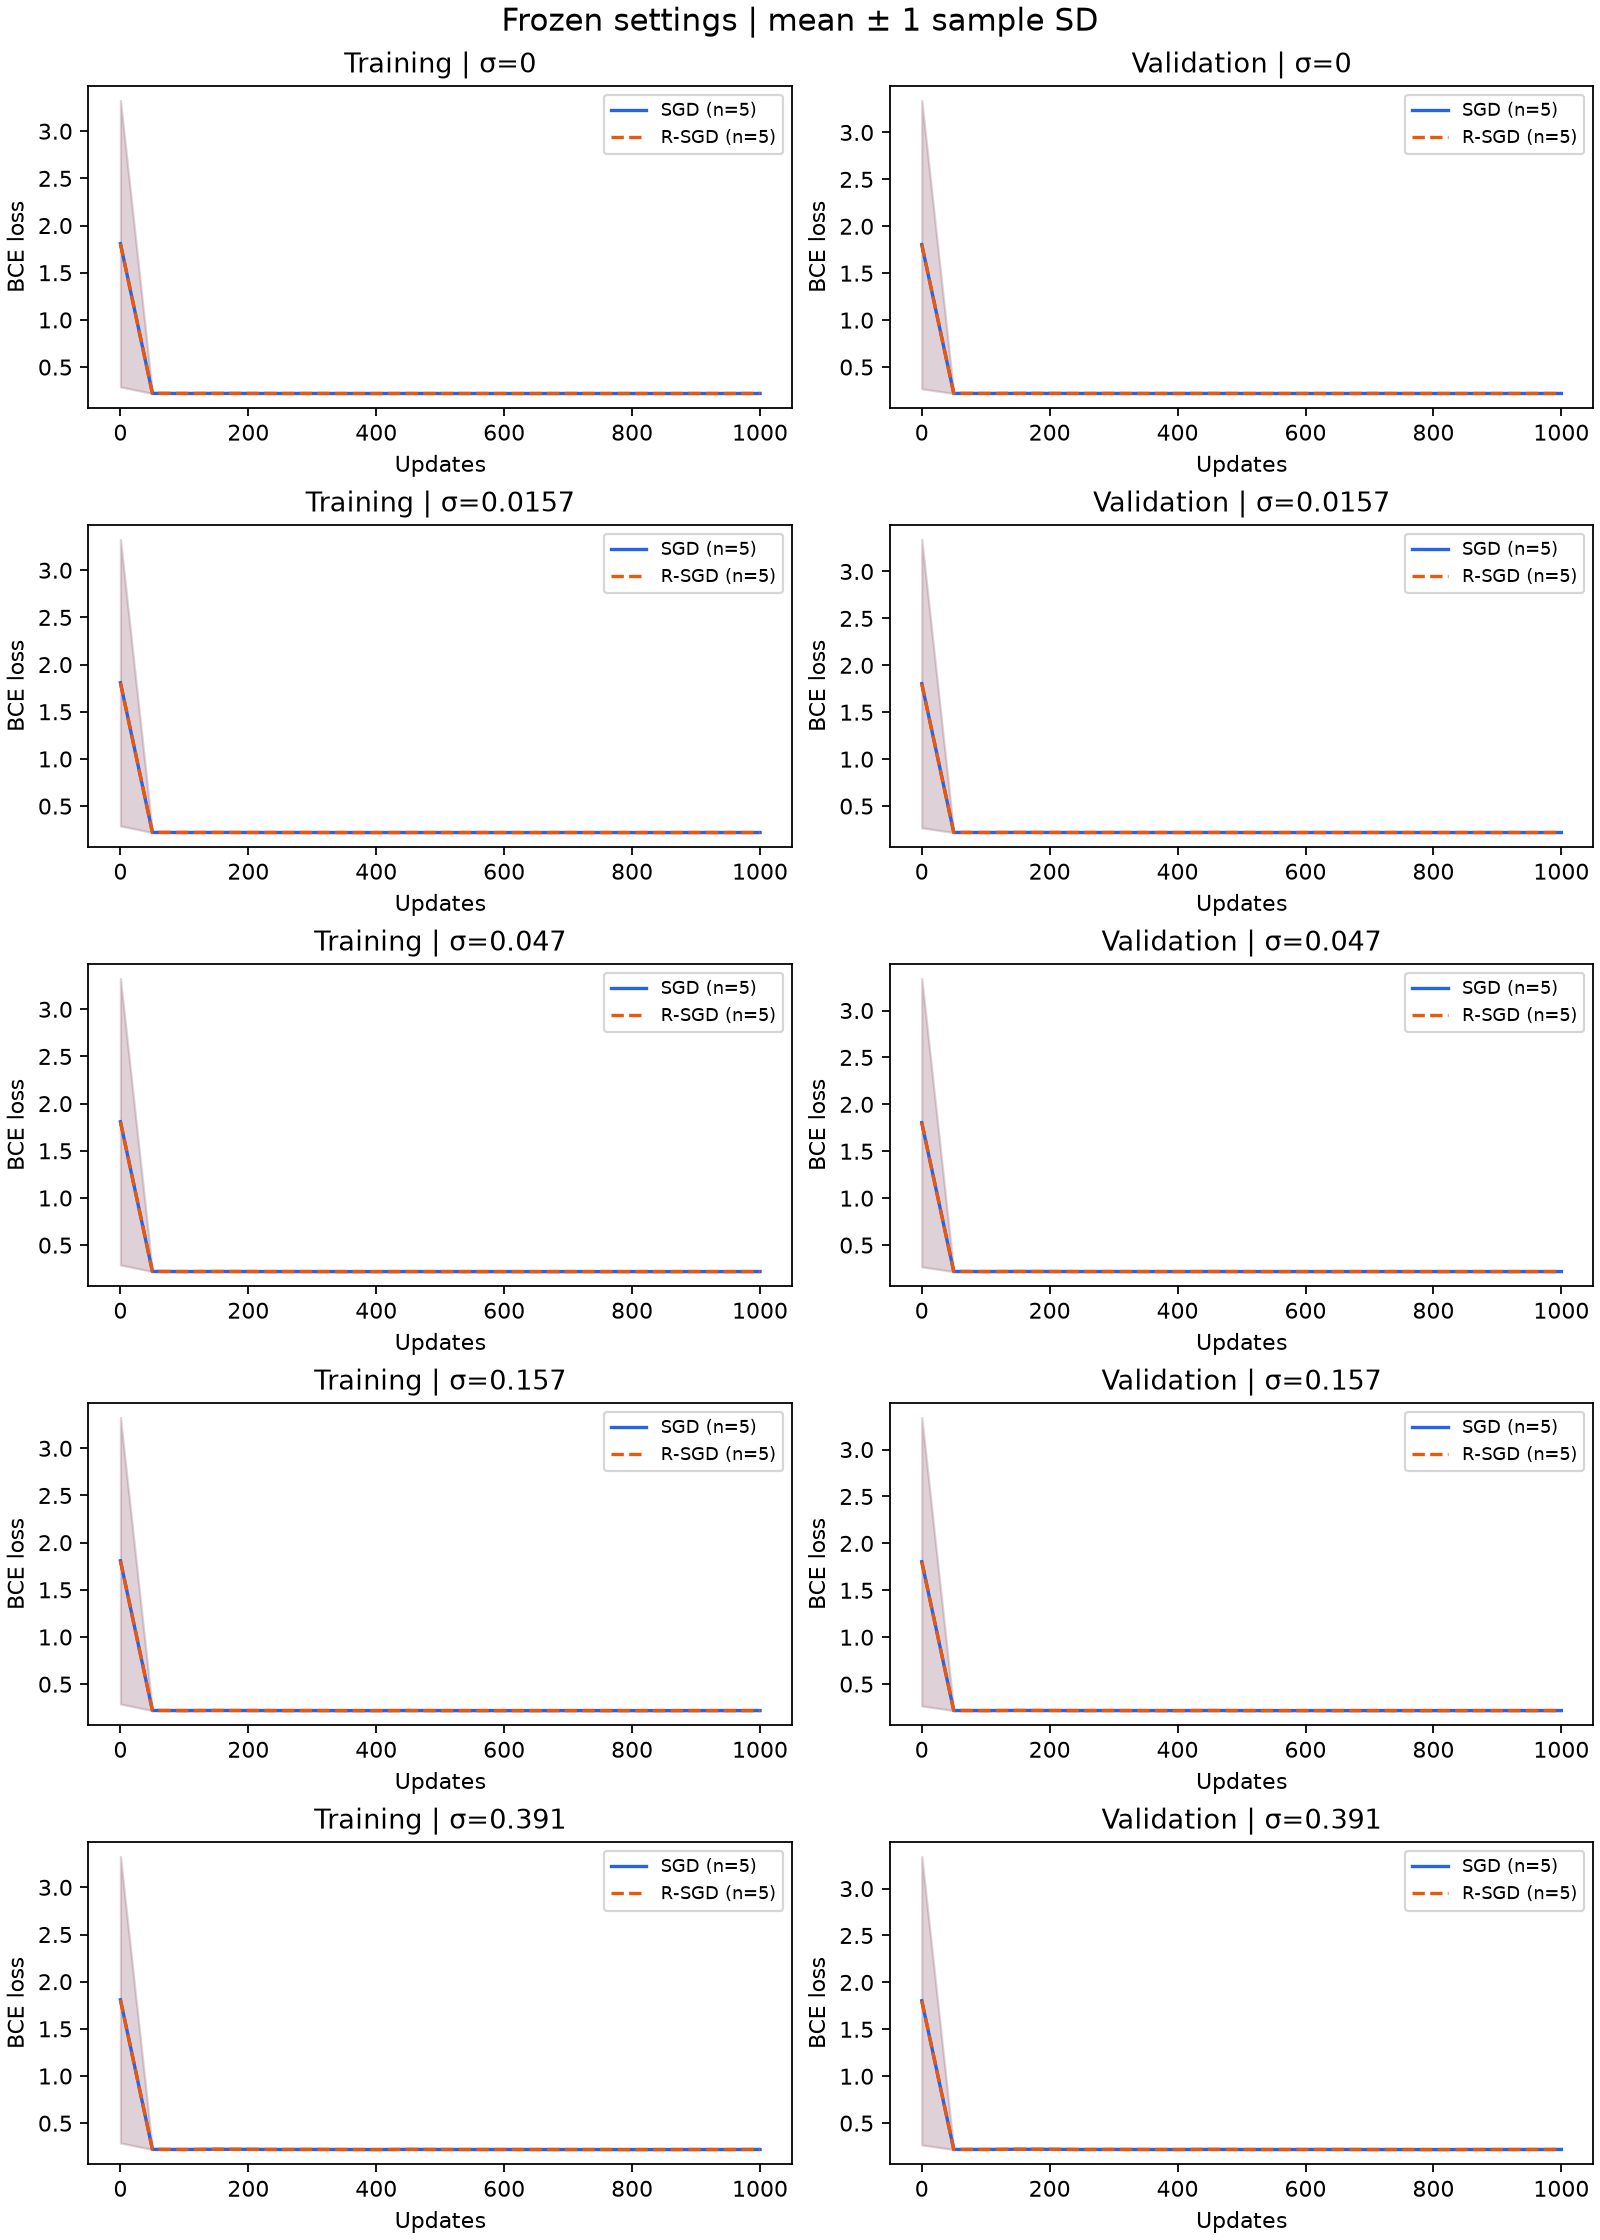
\includegraphics[width=0.9\textwidth]{./plots/logreg/loss_curves.png}
    \caption{Simulation 1 training and validation losses against updates.}
    \label{fig:sim1_loss_curves}
\end{figure}

Figure \ref{fig:sim1_loss_curves} shows that the training process is almost the 
same across different noise levels. All experiments led to approximately the 
same results. The same situation can be seen in Figure \ref{fig:sim1_boundary}: 
despite adding the noise, the model still splits the classes successfully after 
being tuned with ordinary SGD.

However, a detailed analysis of the metrics (presented in Figure 3) reveals several important observations:

\begin{itemize}
    \item As shown in the bottom-middle panel, the 
    number of gradient evaluations remains strictly constant (at 9600) across all 
    noise levels. This confirms that the computational budget is identical for all 
    experiments, ensuring a fair comparison.
    
    \item While the test loss exhibits a visible upward 
    trend as the noise level \(\sigma\) increases, the test accuracy remains highly 
    stable at approximately 0.93. This indicates that standard SGD is robust enough 
    to handle this task even with substantial added gradient noise, successfully 
    finding a decision boundary that generalizes well.
    
    \item The error bars (representing 1 sample SD over 
    5 seeds) widen as \(\sigma\) increases. This is expected: higher levels of 
    artificial gradient noise introduce greater stochasticity into the optimization 
    path, leading to higher variance in the final model parameters.
    
    \item Interestingly, the error bars for the test loss 
    do not show a clear trend of increasing with \(\sigma\). This is logical because 
    the model was never trained on the test data; thus, the test gradients were never 
    computed or corrupted by noise. The test loss simply reflects the evaluation of 
    the trained parameters on clean data.
    
    \item The bottom-right panel confirms that the 
    zero-step frequency is exactly zero across all noise levels. This is expected for 
    standard SGD, where the robustness radius \(\rho = 0\), meaning the optimization 
    step is never intentionally halted.
    
    \item The runtime plot (bottom-left) shows a noticeable 
    spike in variance at \(\sigma \approx 0.15\). Because the computational complexity 
    of the SGD update does not depend on the noise level \(\sigma\), this anomaly is 
    likely an artifact of operating system scheduling or Python garbage collection 
    during those specific runs, rather than an algorithm-specific effect.
\end{itemize}
\begin{figure}[htbp]
    \centering
    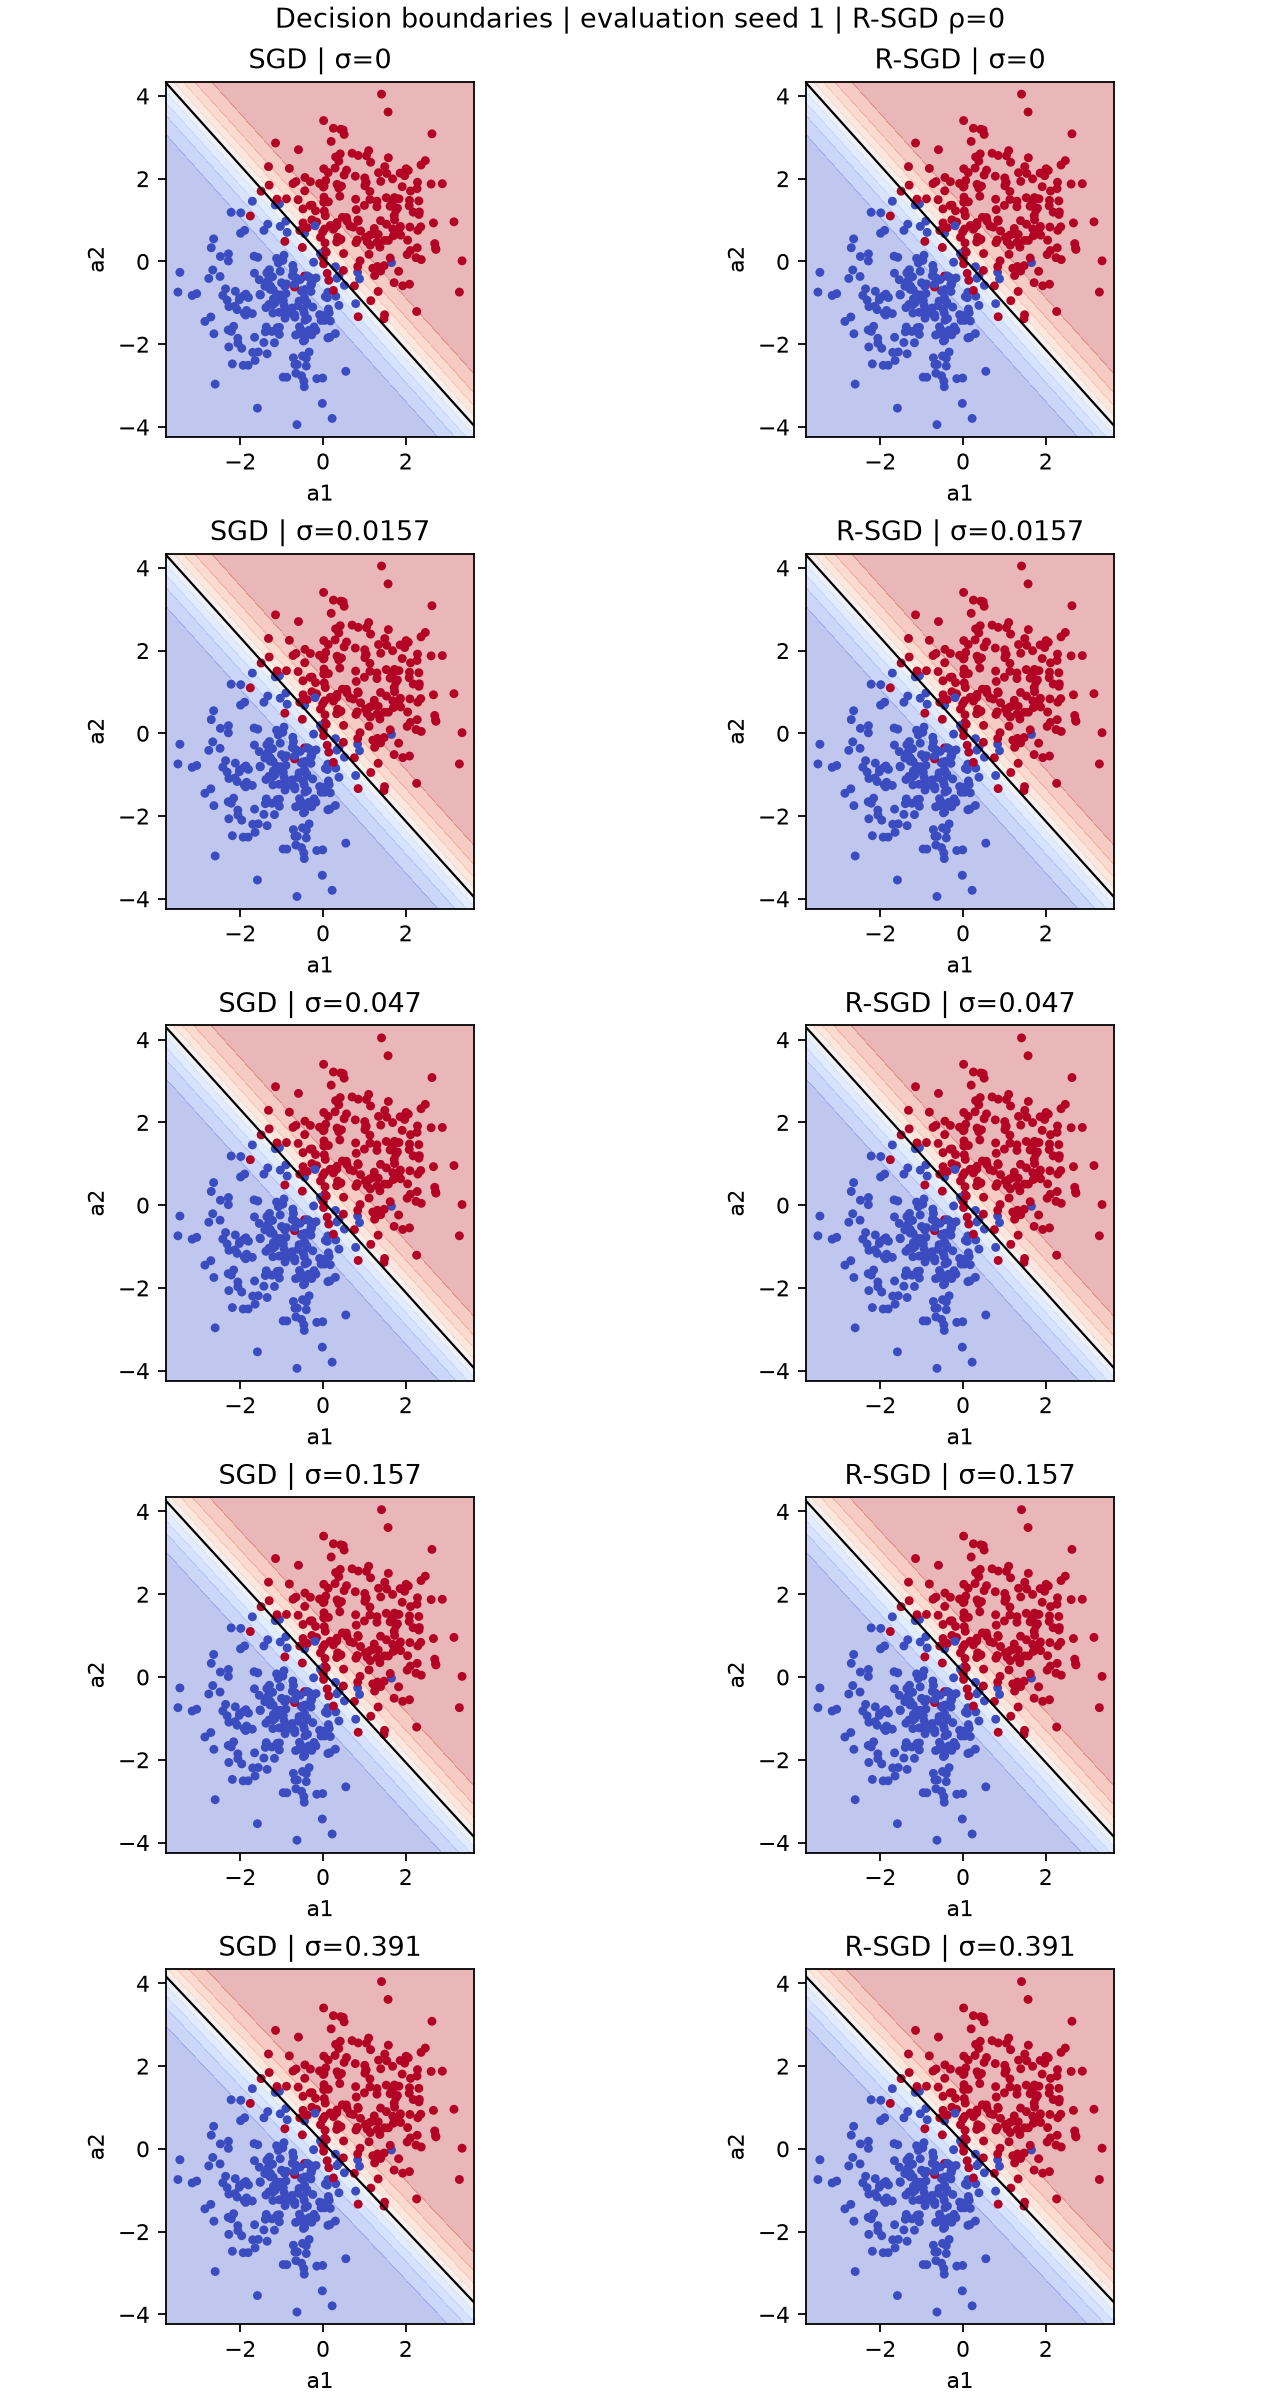
\includegraphics[width=0.95\textwidth]{./plots/logreg/decision_boundaries.png}
    \caption{Decision boundaries for seed=1, for SGD with lr=1.}
    \label{fig:sim1_boundary}
\end{figure}

\begin{figure}[htbp]
    \centering
    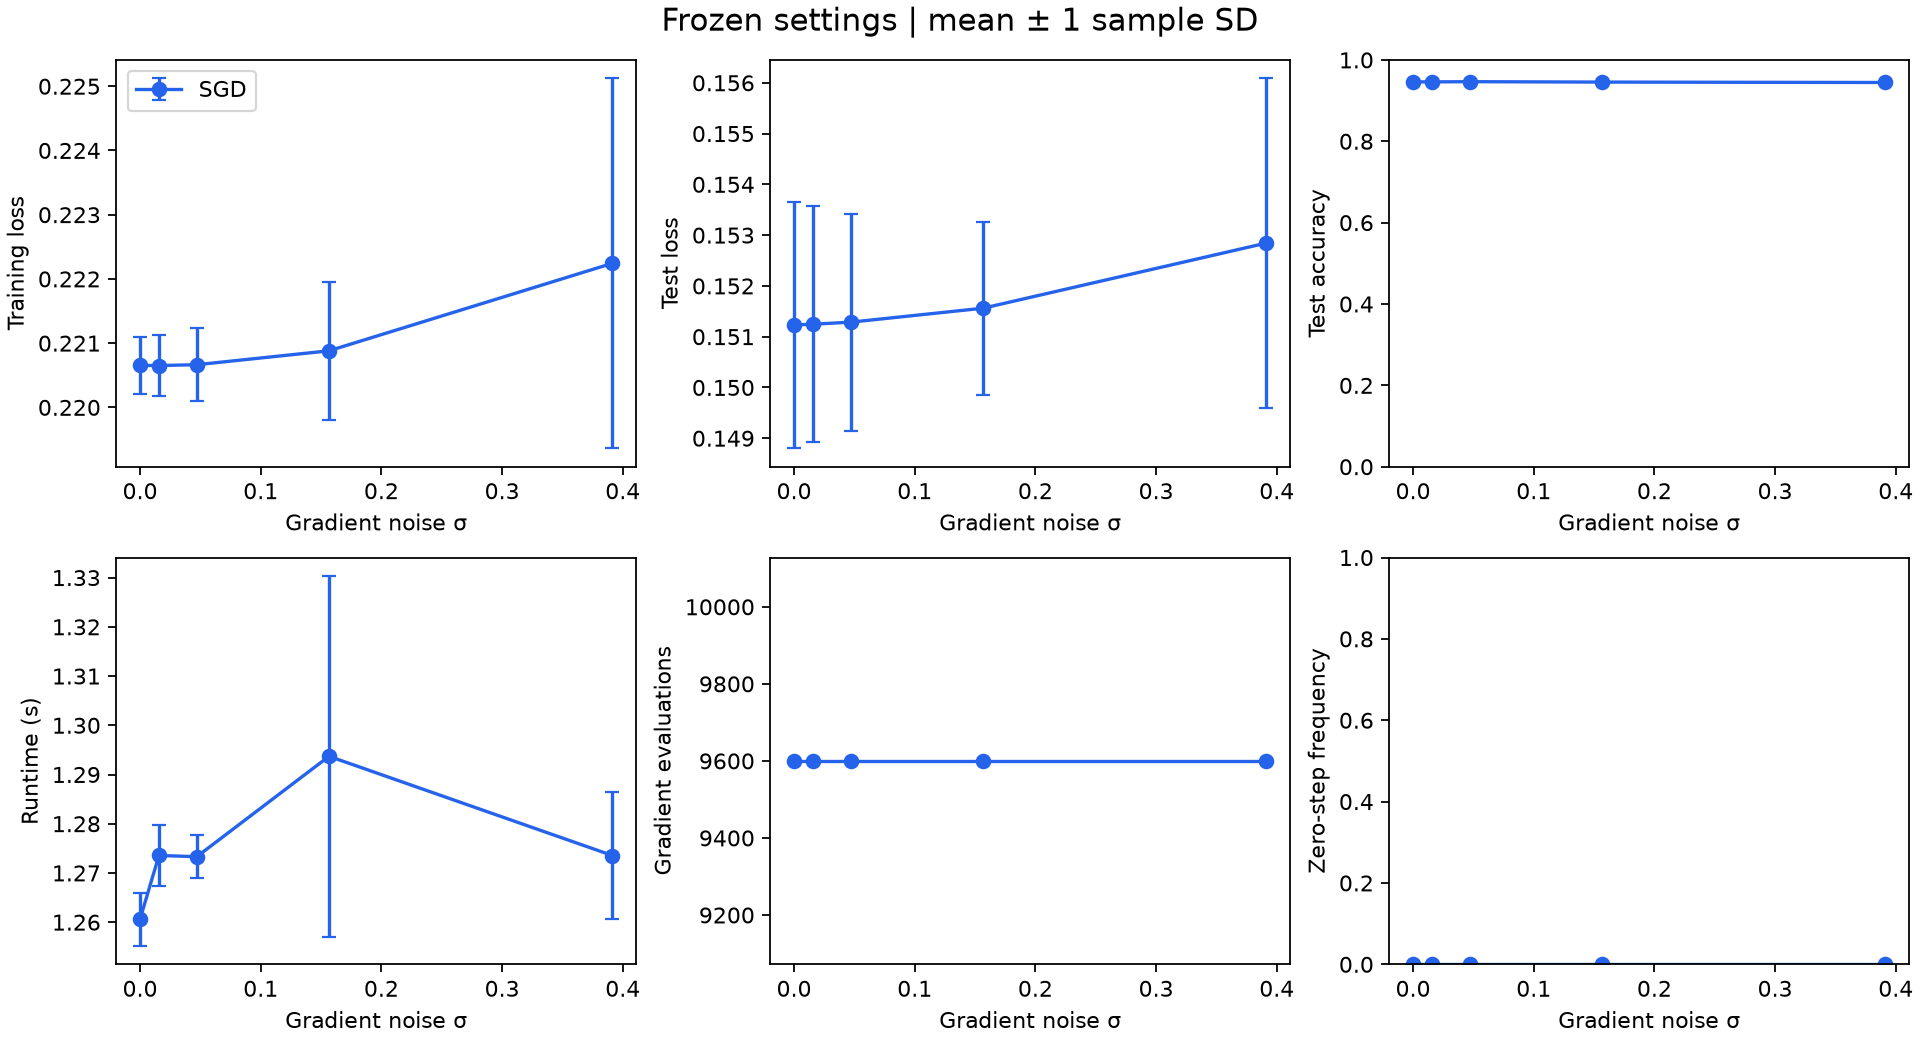
\includegraphics[width=0.9\textwidth]{./plots/logreg/noise_summary.png}
    \caption{Simulation 1 metrics vs. gradient noise \(\sigma\). Mean \(\pm\) 1 sample SD over 5 evaluation seeds. Top row: final training loss, test loss, and test accuracy. Bottom row: runtime, gradient evaluations, and zero-step frequency.}
    \label{fig:sim1_metrics}
\end{figure}


\begin{figure}[htbp]
    \centering
    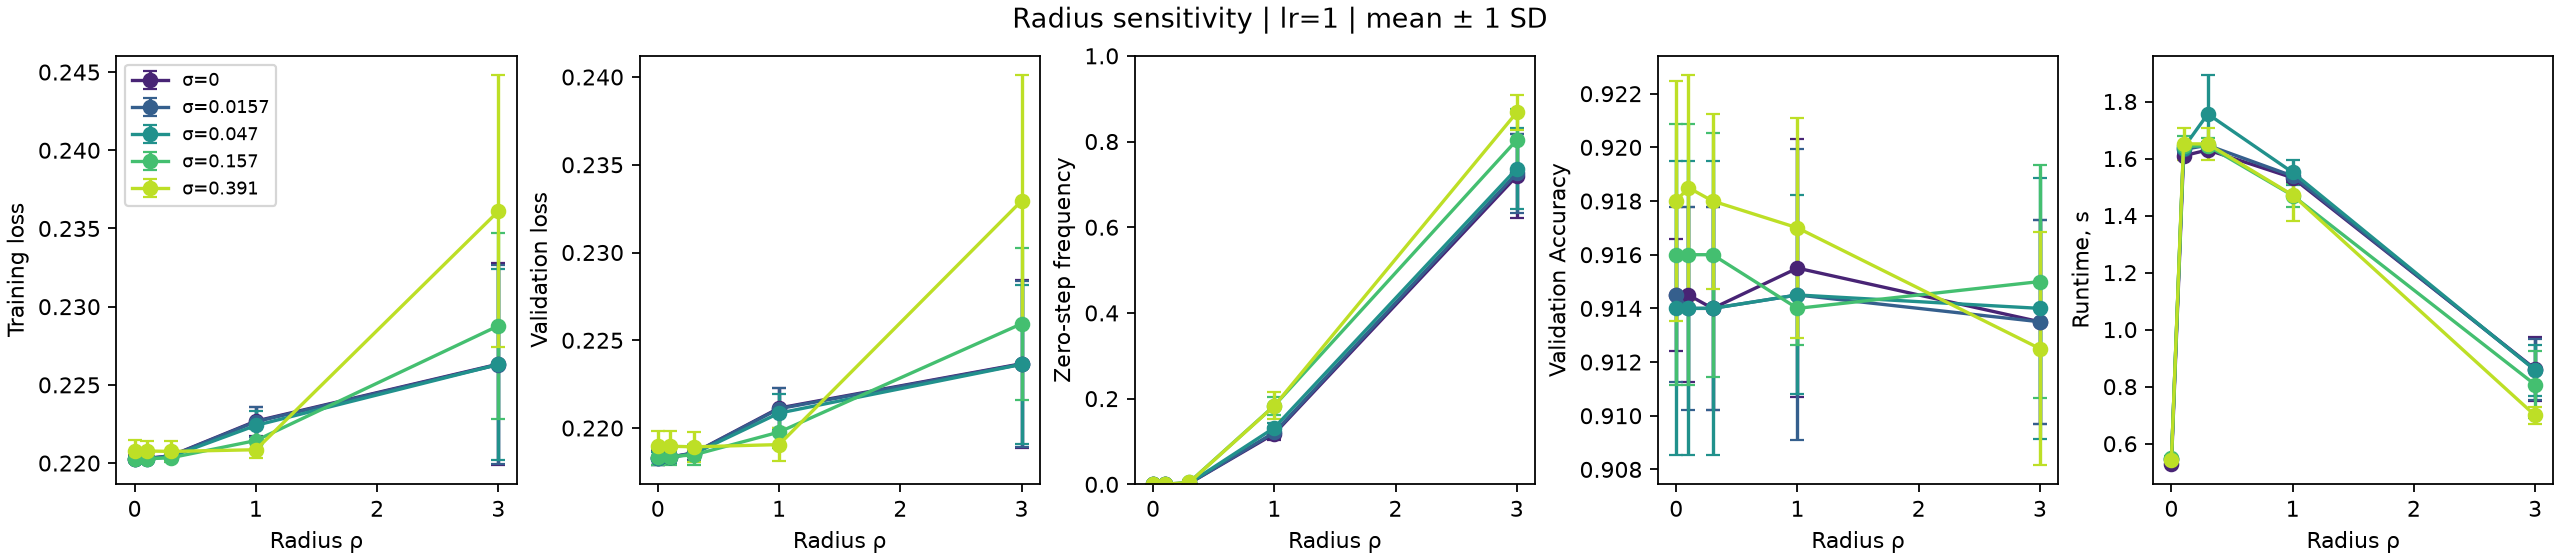
\includegraphics[width=\textwidth]{./plots/logreg/radius_sensitivity.png}
    \caption{Simulation 1 metrics vs radius \(\rho\).}
    \label{fig:sim1_radius}
\end{figure}

\subsection{Sensitivity to Robustness Radius}
\label{sec:sim1_radius}

Figure \ref{fig:sim1_radius} illustrates the impact of varying the robustness radius \(\rho\) (at a fixed learning rate \(lr=1\)) on training loss, validation loss, zero-step frequency, validation accuracy, and runtime.

\begin{itemize}
    \item As the radius \(\rho\) increases, both training and validation losses exhibit a clear upward trend. This degradation is directly linked to the increasing frequency of zero-steps. With a larger radius, the optimizer frequently halts its updates, causing the training process to terminate at a less optimal point compared to configurations with fewer zero-steps.
    
    \item The zero-step frequency increases monotonically with \(\rho\) (reaching over 80\% at \(\rho=3\)). This is mathematically consistent with the zero-step condition derived in the theoretical section:
    \begin{equation}
        g_k^T S_k^{-1} g_k \le \rho^2 \implies d_k = 0.
    \end{equation}
    As \(\rho\) grows, the uncertainty ball expands, making it increasingly likely that the gradient magnitude is "swallowed" by the uncertainty bound, forcing the robust step \(d_k\) to zero.
    
    \item Although the loss worsens significantly with larger \(\rho\), the validation accuracy remains remarkably stable, converging to approximately \(0.91\) across all tested radii. This divergence is due to the fundamental difference between the two metrics: loss is a continuous measure sensitive to even the smallest shift in the decision boundary, whereas accuracy is a discrete metric. Accuracy only changes if the boundary shifts enough to push a data point to the other side of the classification threshold. Therefore, a noticeable increase in loss does not necessarily translate to a drop in accuracy.
    
    \item The runtime behavior reveals an interesting non-monotonic trend: it initially spikes and then decreases as \(\rho\) grows. This is directly correlated with the zero-step frequency. When the zero-step condition is met, the algorithm bypasses the iterative numerical solver for the \(d_k\) subproblem and simply sets the step to zero. The computational savings from skipping the solver eventually outweigh the overhead of computing the covariance matrix \(S_k\), leading to reduced runtime at very large radii.
    
    \item Comparing the optimizers, SGD and R-SGD achieve nearly identical validation accuracy. However, standard SGD is consistently faster than R-SGD (at \(\rho \to 0\)), making it the more computationally efficient choice for this specific task where robustness yields no predictive advantage.
    
    \item The error bars represent one sample standard deviation across the 5 evaluation seeds. The relatively large variance can be attributed to the limited number of seeds and the moderate batch size. This constraint results in fewer explored initializations and higher variance in the per-example gradient estimates at each optimization step.
\end{itemize}

\subsection{Reproducibility}

To reproduce the experiment use \href{https://github.com/Anya497/Optimization_HW1}{our repository}\footnote{\url{https://github.com/Anya497/Optimization_HW1} --- link to repository with experiments code.} and follow the guide in the section "Simulation 1".
